%%%%%%%%%%%%%%%%%%%%%%%%%%%%%%%%%%%%%%%%%%%%%%%%%%%%%%%%%%%%
%%%%%%%%%%%%%%%%%%%%%%%%%%%%%%%%%%%%%%%%%%%%%%%%%%%%%%%%%%%%
%%%%%%%%%%%%%%%%%%%%%%%%%%%%%%%%%%%%%%%%%%%%%%%%%%%%%%%%%%%%
\section{Weighted Residual Formulation}
%%%%%%%%%%%%%%%%%%%%%%%%%%%%%%%%%%%%%%%%%%%%%%%%%%%%%%%%%%%%
%%%%%%%%%%%%%%%%%%%%%%%%%%%%%%%%%%%%%%%%%%%%%%%%%%%%%%%%%%%%
%%%%%%%%%%%%%%%%%%%%%%%%%%%%%%%%%%%%%%%%%%%%%%%%%%%%%%%%%%%%

\subsection{Abstract Formulation}

When we go about to solve a PDE problem we need a general idea of what
a PDE problem is. We will develop such an idea in this section.

\begin{frame}
\frametitle<presentation>{Weighted Residual Formulation}
\begin{Def}[Weighted Residual Formulation]
We claim that all problems we ever want to solve can be written in the form
\begin{equation}
\text{Find } u_h\in w_h + \tilde{U}_h : \qquad r_h(u_h,v) =
0 \qquad \forall v\in \tilde{V}_h.  
\end{equation}
Where:
\begin{itemize}
\item $\tilde{U}_h\subseteq U_h$, $\tilde{V}_h\subseteq V_h$ are
finite-dimensional function spaces and corresponding subspaces.
\item Affine shift: $u_h\in w_h + \tilde{U}_h$ for a given $w_h\in U_h$ means
$u_h = w_h + \tilde{u}_h$ for some $\tilde{u}_h\in\tilde{U}_h$.
\item $r_h : U_h \times V_h \to \mathbb{K}$ is the \textit{residual form}.
\begin{itemize}
\item $r_h$ may be \textit{nonlinear} in its first argument.
\item $r_h$ \textit{is always linear} in its second argument.
\item $r_h$ may depend on the grid in non-conforming methods.
\end{itemize}
\item We assume that this problem has a unique solution. \hfill$\square$
\end{itemize}
\end{Def}
\end{frame}

We now give some concrete examples.

\subsection{Some Examples}

\paragraph{Continuous Problem}

\begin{frame}
\frametitle<presentation>{Continuous Problem}

Consider the Poisson equation
\begin{subequations}
\label{Eq:DiffusionEquation}
\begin{align}
                -\Delta u &= f& \text{in }& \Omega\subseteq\mathbb{R}^n,\\
                        u &= g& \text{on }& \Gamma_D\subseteq\partial\Omega,\\
     - \nabla u\cdot\nu   &= j& \text{on }& \Gamma_N=\partial\Omega\setminus\Gamma_D,
\end{align}
\end{subequations}
where $\mbox{meas}(\Gamma_D)\neq 0$. 

The \textit{weak formulation} uses the spaces
\begin{equation*}
U = H^1(\Omega), \qquad
\tilde{U} = \{u \in U\,|\, \text{``$u=0$'' on $\Gamma_D$}
\}
\end{equation*}
and reads
\begin{equation}\label{Eq:DiffusionWeakForm}
u \in w+\tilde{U} \  : \quad
\underbrace{\int_\Omega \nabla u \cdot \nabla v \diffd x
+ \int_{\Gamma_N} j v \diffd s - \int_\Omega f v \,dx}_{= r(u,v)} = 0,  
\quad \forall v\in \tilde{U}.
\end{equation}
Here $w\in U$ is a function with ``$w=g$'' on $\Gamma_D$ and $V=U$, $\tilde{V}=\tilde{U}$.
\end{frame}


\paragraph{Conforming Finite Elements of Order $k$}

First we need to introduce some notation for the grid:

\begin{frame}
\frametitle<presentation>{Conforming Finite Elements of Order $k$}
$\mathbb{T}_h$ is a grid with elements
$E_h^0=\{e_0,\ldots,e_{N_h^0-1}\}$
covering the domain $\Omega\subset\mathbb{R}^n$.

$\Omega_e$ is the domain (open, connected set) associated with element
$e\in E_h^0$.

The discrete function spaces now are
\begin{align*}
U_h^k &= \{u\in C^0(\Omega) \,|\, u|_{\Omega_e}\in P_k
\}, &
\tilde{U}_h^k &= \{u \in U_h^k \,|\, \text{``$u(x) = 0$'' for $x\in\Gamma_D$}\}.
\end{align*}
$P_k$ are the polynomials of degree $k$ and $\Gamma_D$ is resolved
by the mesh.

Now take $w_h\in U_h^k$ with ``$w_h(x) = g(x)$'' (sample at vertices)
on $\Gamma_D$ and find $u_h\in w_h+\tilde{U}_h^k$ s.t.  
\begin{equation}
\underbrace{\sum_{e\in E_h^0}\int_{\Omega_e} \nabla u_h \cdot \nabla v \diffd x
 + \sum_{\substack{b\in B^1_h\\ \Omega_b\subseteq\Gamma_N}} 
\int_{\Omega_b} j v \diffd s - \sum_{e\in E_h^0} \int_{\Omega_e} f v \,dx}_{= r^\text{FE}_h(u,v)}
 = 0 \qquad \forall v\in \tilde{U}^k_h.
\end{equation}
Obviously, we have $r^\text{FE}_h(u_h,v) = r(u_h,v)$.
\end{frame}

\paragraph{Vertex-centered Finite Volumes}

This method uses a discontinuous test space that is constant on
``cells''. Let us introduce some notation to define this formally.

\begin{frame}<article>
\frametitle<presentation>{Vertex-centered Finite Volumes}
\begin{window}[0,r,{
\psfrag{bi}{$c_i$}
\psfrag{vi}{$z_i$}
\psfrag{bj}{$c_j$}
\psfrag{vj}{$z_j$}
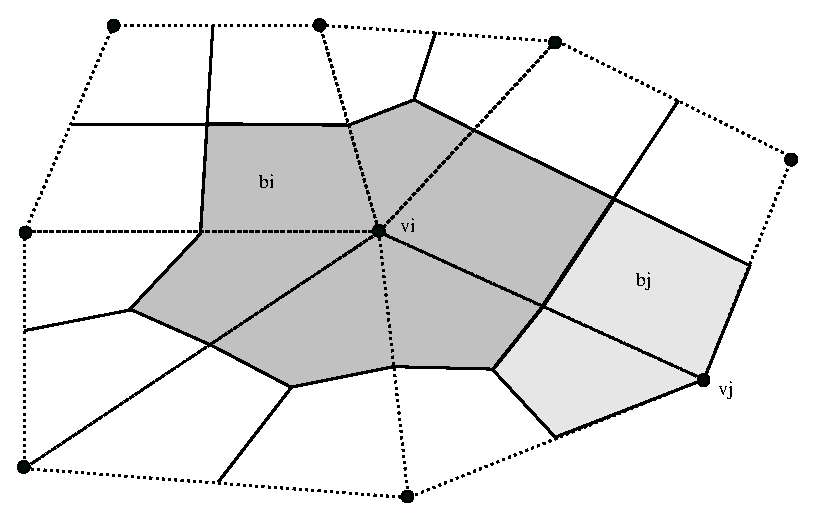
\includegraphics[width=0.4\textwidth]{./EPS/SecMesh2D}},{}]
$E_h^d=\{z_0,\ldots,z_{N_h^d-1}\}$ are the vertices of the mesh
(entities of codimension $d$). 

$x_z$ is the position of $z\in E_h^d$.

$C_h = \{c_0,\ldots,c_{N_h^d-1}\}$ are ``cells'' around each vertex of
the mesh.
\end{window}

$\Omega_c$ is the domain of $c\in C_h$ and $x_c=x_z$ when $c$ is the
cell around $z$.

Define the \textit{discontinuous} test function space:
\begin{align*}
V_h^0 & = \{ v\in L_2(\Omega) \,|\, \forall c\in C_h : v|_{\Omega_c} =
\text{const} \},\\
\tilde{V}_h^0 &= \{ v\in V_h \,|\, \forall z\in E_h^d, x_z\in\Gamma_D : v(x_z)=0\}.
\end{align*}

\end{frame}

\begin{frame}<article>
\frametitle<presentation>{Vertex Centered Finite Volumes (Contd.)}
The discontinuities are located on the \textit{skeleton} which is given by:
\begin{equation*}
\Gamma_h^{\text{int}} = \{\gamma_{e,c,c^\prime} \,|\,
\gamma_{e,c,c^\prime} = \Omega_e \cap \partial\Omega_c \cap
\partial\Omega_{c^\prime} \}
\end{equation*}
and the boundary faces are given by
\begin{equation*}
\Gamma_h^{\text{ext}} = \{\gamma_{e,c} \,|\,
\gamma_{e,c} = \partial\Omega_e \cap \partial\Omega_c \cap
\partial\Omega \}.
\end{equation*}

For $\gamma\in\Gamma_h^{\text{int}}$, $\nu_\gamma(x)$ is
the \textit{unique} unit
normal vector to $\gamma$ in point $x$. 

Similarly, for
$\gamma\in\Gamma_h^{\text{ext}}$, $\nu_\gamma(x)$ is the unit outer
normal vector.

The jump of a function $v\in V_h$ in
$x\in\gamma\in\Gamma_h^{\text{int}}$ given by
\begin{equation*}
[v]_\gamma(x) = \lim_{\varepsilon\to 0-} v(x+\varepsilon \nu_\gamma(x))
-  \lim_{\varepsilon\to 0+} v(x+\varepsilon \nu_\gamma(x))\quad.
\end{equation*}
\end{frame}

\begin{frame}<article>
\frametitle<presentation>{Vertex Centered Finite Volumes (Contd.)}
The discrete problem then reads as follows. Find $u_h\in w_h+\tilde{U}_h^1$ s.t.
\begin{equation}
\underbrace{- \sum_{\gamma\in\Gamma_h^{\text{int}}} \int_\gamma
\nabla u_h \cdot \nu_\gamma \,[v]\diffd s
+ \sum_{\substack{\gamma\in\Gamma_h^{\text{ext}},\\ \gamma\subseteq\Gamma_N}}
\int_\gamma j v \diffd s\quad
- \int_\Omega fv \diffd x}_{= r_h^\text{FE}(u_h,v)} = 0,
\quad \forall v\in \tilde{V}_h^0.
\end{equation}
$\tilde{U}_h^1$ is the linear conforming finite element space and $w_h$ is
defined as before.

Typically, the integrals are evaluated with low order quadrature rules
such as the midpoint rule.

This gives a simple example with non-conforming residual form and
different trial and test functions.
\end{frame}


\paragraph{Cell Centered Finite Volumes}

\begin{frame}<article>
\frametitle<presentation>{Cell Centered Finite Volumes}
Assume that $\mathbb{T}_h$ is either a Delauney
triangulation or a structured cube mesh.

$E^1_h = \{f_0,\ldots,f_{N^1_h-1}\}$ is the set of interior
faces (intersections of two \textit{elements}).

$B^1_h = \{b_0,\ldots,b_{NB^1_h-1}\}$ is the set of exterior faces
(intersections of elements with the domain boundary).

$l,r : E^1_h \to E^0_h$ deliver the ``left'' and ``right'' elements for an
interior face. 

$\nu_f$ denotes the unit normal vector to $f\in E^1_h$ that points from
$l(f)$ to $r(f)$.

Similarly, $l : B^1_h \to E^0_h$ gives the element where $b\in B_h$ is a
face of and $\nu_b$ is the unit outer normal.
\end{frame}

%$\Omega_f$ is the domain of $f\in E_h^1, B_h^1$, $x_f$ is its center.

%$\omega_e = \text{interior}(\overline{\omega_{l(e)}\cup
%\omega_{r(e)}})$ is the domain of the two elements adjacent to $e\in
%E_h$.

%$\omega_b = \omega_{l(e)}$. 

\begin{frame}
\frametitle<presentation>{Cell Centered Finite Volumes (Contd.)}
Define space of \textit{element-wise} constant functions:
\begin{equation*}
W_h^0 = \{  u\in L_2(\Omega) \,|\, \forall e\in E^0_h : u|_{\Omega_e} =
\text{const} \} .
\end{equation*}

The discrete problem then reads
\begin{equation*}
u_h\in W_h^0 \ : \ r_h^\text{CC}(u_h,v) = 0 \quad \forall v\in W^0_h
\end{equation*}
where
\begin{equation*}
\begin{split}
r_h^\text{CC}(u,v) &= \sum_{f\in E^1_h} \int_{\Omega_f}
\frac{u(x_{l(f)})-u(x_{r(f)})}{\|x_{r(f)}-x_{l(f)}
\|}\,[v]\diffd s
+ \sum_{\substack{b\in B^1_h\\ \Omega_b\subseteq\Gamma_D}} \int_{\Omega_b}
\frac{u(x_{l(b)})-g(x_b)}{\|x_{b}-x_{l(b)}\|}\, v \diffd s \\
& \qquad - \sum_{e\in E_h^0} \int_{\Omega_e} fv \diffd x -
\sum_{\substack{b\in B^1_h\\ \Omega_b\subseteq\Gamma_N}}
\int_{\Omega_b} j v \diffd s .
\end{split}
\end{equation*}

Note that in this formulation there are no essential boundary
conditions. 
\end{frame}

\paragraph{Discontinuous Galerkin}

\begin{frame}<article>
\frametitle<presentation>{Discontinuous Galerkin Finite Element
Method}
Let $k : E^0_h \to \mathbb{N}_0$ be a function that associates an
nonnegative integer with each element.

Define the discrete function space
\begin{equation*}
W_h^k = \{u\in L_2(\Omega) \,|\, \forall e\in E^0_h : u|_{\Omega_e} \in P_{k(e)}\}.
\end{equation*}

For any $x\in\Omega_f, f\in E_h^1$, define the jump of a function
$u\in W_h^k$:
\begin{equation*}
\label{Eq:Jump}
[u]_f(x) = \lim\limits_{\epsilon\to 0-} u(x+\epsilon\nu_f) - 
\lim\limits_{\epsilon\to 0+} u(x+\epsilon\nu_f).
\end{equation*}

For any $x\in\Omega_f, f\in E_h^1$, define the average of a function
$u\in W_h^k$:
\begin{equation*}
\label{Eq:Average}
\langle u\rangle_f(x) = \frac{1}{2}\left(\lim\limits_{\epsilon\to 0-} u(x+\epsilon
\nu_f) +  \lim\limits_{\epsilon\to 0+} u(x+\epsilon
\nu_f)\right ).
\end{equation*}

\end{frame}


\begin{frame}
\frametitle<presentation>{Discontinuous Galerkin Finite Element
Method (Contd.)}
The discrete problem for the OBB method \cite{OBB98} then reads
\begin{equation*}
u_h \in W^k_h \quad : \quad r_h^\text{OBB}(u_h,v) = 0 \qquad \forall v\in W_h^k,
\end{equation*}
where
\begin{equation*}
\begin{split}
r_h^\text{OBB}(u &,v) = \sum_{e\in E_h^0} \int_{\Omega_e} \nabla u\cdot \nabla v
 - fv \, dx \\
&+ \sum_{f\in E^1_h} \int_{\Omega_f} \langle \nabla v\cdot\nu_f\rangle [u]_f
- [v]_f \langle \nabla u\cdot \nu_f\rangle \, ds\\
&+ \sum_{\substack{b\in B^1_h\\\Omega_b\subseteq\Gamma_D}} \int_{\Omega_b} (\nabla v\cdot\nu_f) (u-g)
- v (\nabla u\cdot \nu_f) \, ds + \sum_{\substack{b\in
B^1_h\\\Omega_b\subseteq\Gamma_N}} \int_{\Omega_b} j v \,ds .
\end{split}
\end{equation*}
Note the seperation into volume, skeleton and boundary terms.
\end{frame}


\paragraph{Crouzeix-Raviart}

\begin{frame}
\frametitle<presentation>{Crouzeix-Raviart Element}
Here we use the following discrete spaces:
\begin{align*}
X_h &= \{u\in L_2(\Omega) \,|\, u|_{\Omega_e}\in P_1 \text{ and $u$
continuous at face centers}\},\\
\tilde{X}_h &= \{u\in X_h \,|\, \text{``$u=0$'' on $\Gamma_D$}\}.
\end{align*}

The discrete problem then reads
\begin{equation*}
u_h \in w_h+\tilde{X}_h \quad : \quad r_h^\text{CR}(u_h,v) = 0 \qquad \forall v\in \tilde{X}_h,
\end{equation*}
where
\begin{equation*}
\begin{split}
r_h^\text{CR}(u &,v) = \sum_{e\in E_h^0} \int_{\Omega_e} \nabla u\cdot \nabla v \, dx
+ \sum_{\substack{b\in
B^1_h\\\Omega_b\subseteq\Gamma_N}} \int_{\Omega_b} j v \,ds  - \sum_{e\in E_h^0} \int_{\Omega_e} fv \, dx .
\end{split}
\end{equation*}
Again $w_h\in X_h$ such that ``$w_h=g$'' on $\Gamma_D$.
\end{frame}

\paragraph{Mixed Finite Elements}

\begin{frame}<article>
\frametitle<presentation>{Mixed Finite Element Method}
Defining the ``flux'' $\sigma=-\nabla u$ we rewrite problem
\eqref{Eq:DiffusionEquation} as a system of first order equations:
\begin{subequations}
\label{Eq:DiffusionEquationMixedForm}
\begin{align*}
\sigma + \nabla u &= 0 & \text{in }& \Omega\subseteq\mathbb{R}^n,\\
\nabla \cdot \sigma     &= f & \text{in }& \Omega,\\
                      u &= g& \text{on }& \Gamma_D\subseteq\partial\Omega,\\
        \sigma\cdot\nu  &= j& \text{on }& \Gamma_N=\partial\Omega\setminus\Gamma_D.
\end{align*}
\end{subequations}
\end{frame}

\begin{frame}<article>
\frametitle<presentation>{Mixed Finite Element Method (Contd.)}
For the flux we introduce the function space
\begin{subequations}
\begin{align*}
S &= H(\text{div};\Omega) = \{\sigma\in \left(L_2(\Omega)\right)^d \,|\,
\nabla\cdot \sigma \in L_2(\Omega)\},\\
\tilde{S} &= \{\sigma\in S \,|\, \text{``$\sigma\cdot\nu=0$'' on $\Gamma_N$} \}
\end{align*}
\end{subequations}
Note that the Neumann boundary conditions are now the essential
boundary conditions built into the function space.  

Using integration by parts we arrive at the weak formulation of the continuous problem.

Find $(\sigma,u)\in (w+\tilde{S})\times L_2(\Omega)$ s. t.
\begin{align*}
\int\limits_\Omega \sigma\cdot v \, dx  -\int\limits_\Omega
u \, \nabla\cdot v \, dx & =  
-\int\limits_{\Gamma_D} g v\cdot \nu \, ds 
& \forall v &\in \tilde{S}\\
- \int\limits_\Omega \nabla\cdot\sigma \, q \, dx      &= 
- \int\limits_\Omega f q \, ds &
\forall q &\in L_2(\Omega)
\end{align*}
where $w\in S :$ ``$w\cdot\nu = j$'' on $\Gamma_N$.
\end{frame}

\begin{frame}<article>
\frametitle<presentation>{Mixed Finite Element Method (Contd.)}
For discretization use finite dimensional subspaces
of the involved function spaces. 
E.g. the Raviart-Thomas space of lowest order on triangles:
\begin{align*}
S_h &= \left\{\sigma\in\left(L_2(\Omega) \right)^2  \,\Bigl|\, \sigma|_{\Omega_e} =
\left(\begin{array}{l} a_e\\ b_e \end{array}\right) + 
c_e \left(\begin{array}{l} x\\ y \end{array}\right) \quad\forall e\in E^0_h
\right\} .
\end{align*}

Then the discrete problem in residual form reads:
\begin{equation*}
(\sigma_h, u_h) \in (w_h+\tilde{S}_h)\times W_h^0 : \quad 
r_h^\text{MFE}\left((\sigma_h,u_h),(v,q)\right) = 0 \quad \forall
(v,q) \in \tilde{S}_h\times W_h^0 .
\end{equation*}
with
\begin{equation*}
\begin{split}
r_h^\text{MFE}((\sigma,u)&,(v,q)) = 
\int\limits_\Omega \sigma\cdot v \, dx  -\int\limits_\Omega
u \, \nabla\cdot v \, dx 
 - \int\limits_\Omega \nabla\cdot\sigma \, q \, dx\\ 
&\quad + \int\limits_{\Gamma_D} g v\cdot \nu \, ds + \int\limits_\Omega f q \,
ds .
\end{split}
\end{equation*}
Note: Systems of PDEs lead to tensor product function spaces.
\end{frame}

\subsection{Properties of the Residual Form}

The examples above imply the following properties of $r_h$.

\begin{frame}
\frametitle<presentation>{Properties of the Residual Form}
\begin{Pro}[Splitting]
$r_h$ can be split into element, skeleton and boundary sums
\begin{equation*}
r_h(u,v) = \sum_{e\in E^0_h} r^\text{vol}_{h,e}(u,v) + \sum_{f\in E^1_h} r^\text{skel}_{h,f}(u,v)
+ \sum_{b\in B^1_h} r^\text{bnd}_{h,b}(u,v)
\end{equation*}
$r_h$ can be split into a part depending
on $u$ and a part independent of $u$:
\begin{equation*}
r_h(u,v) = \alpha_h(u,v) + \lambda_h(v) .
\end{equation*}

Together we obtain
\begin{equation}
\begin{split}
r_h(u,v) &= \sum_{e\in E^0_h} \alpha^\text{vol}_{h,e}(u,v) + \sum_{f\in E^1_h} \alpha^\text{skel}_{h,f}(u,v)
+ \sum_{b\in B^1_h} \alpha^\text{bnd}_{h,b}(u,v)\\
&\quad + \sum_{e\in E^0_h} \lambda^\text{vol}_{h,e}(v) + \sum_{f\in E^1_h} \lambda^\text{skel}_{h,f}(v)
+ \sum_{b\in B^1_h} \lambda^\text{bnd}_{h,b}(v) .
\end{split}
\end{equation}
\hfill$\square$
\end{Pro}
\end{frame}

\begin{frame}
\frametitle<presentation>{Properties of the Residual Form (Contd.)}
\begin{Pro}[Linearity]\label{Ass:Linearity}
$r_h$, as well as, $r^\text{vol}_{h,e}$, $r^\text{skel}_{h,f}$ and
$r^\text{bnd}_{h,b}$ are linear in their second
argument.

As a consequence we have $r_h(u,0)=0$.\hfill$\square$
\end{Pro}
\begin{Pro}[Localization]
We assume that the following holds:
\begin{subequations}
\begin{align*}
e&\in E^0_h : & r^\text{vol}_{h,e}(u,v) &= r^\text{vol}_{h,e}(\chi_{\Omega_e} u,\chi_{\Omega_e} v),\\
f&\in E^1_h : & r^\text{skel}_{h,f}(u,v) &=
r^\text{skel}_{h,f}(\chi_{\Omega_{l(f)}\cup\Omega_{r(f)}}
u,\chi_{\Omega_{l(f)}\cup\Omega_{r(f)}} v),\\ 
b&\in B^1_h : & r^\text{bnd}_{h,b}(u,v) &= r^\text{bnd}_{h,b}(\chi_{\Omega_{l(b)}} u,\chi_{\Omega_{l(b)}} v).
\end{align*}
\end{subequations}
where $\chi_\omega(x) : \omega \to \{0,1\}$ is the characteristic function of $\omega$.

This is a consequence of  $r^\text{vol}_{h,e}$, $r^\text{skel}_{h,e}$
and $r^\text{bnd}_{h,e}$ being integrals over an element, a face or a
boundary face.
\end{Pro}
\end{frame}


\subsection{Time-dependent Problems}

What about time-dependent problems?

\begin{frame}
\frametitle<presentation>{Time-dependent problems}
After semidiscretization in space we obtain a problem of the form
\begin{equation*}
u_h(t)\in U_h : \quad \frac{\partial}{\partial t} m_h(u_h(t),v;t) + q_h(u_h(t),v;t)
= 0 \qquad \forall v\in V_h, t\in\Sigma. 
\end{equation*}
Implicit Euler (e.g.) then leads to: Find $u_h^{k+1}\in U_h$ s.t.
\begin{equation*}
\underbrace{m_h(u_h^{k+1},v;t^{k+1}) - m_h(u_h^{k},v;t^k) + \Delta
t^{k}q_h(u_h^{k+1},v;t^{k+1})}_{r_h^\text{IE}(u_h,v)}  = 0
\quad v\in V_h.
\end{equation*}

Explicit Euler (e.g.) leads to: Find  $u_h^{k+1}\in U_h$ s.t.
\begin{equation*}
\underbrace{m_h(u_h^{k+1},v;t^{k+1}) - m_h(u_h^{k},v;t^k) + \Delta
t^{k}q_h(u_h^{k},v;t^{k})}_{r_h^\text{EE}(u_h,v)}  = 0
\quad v\in V_h.
\end{equation*}
Higher-order time discretizations lead to similar problems.

Explicit schemes may lead to easily invertible algebraic systems.
\end{frame}

\cleardoublepage
